\documentclass[a4paper,12pt]{tufte-handout}
\usepackage[utf8]{inputenc}
\usepackage{graphicx}
\usepackage{float}
\usepackage{amsmath}
\usepackage{listings}

\usepackage{setspace}
\doublespacing

\usepackage{hyperref}

\title{Are we behind?\\ \large Scots College IB Students against the World}
\author{Terry Qi}

\begin{document}
\maketitle

\begin{abstract}
    We gather the mark of Year 12 IB students and put them against the IBO collected global values. Its respective mean, median, deviation, and distribution are analyzed and relationships are explored along with some interesting findings when put against itself and others. We conclude with a null hypothesis test with the data to determine the sampling population.
\end{abstract}

\section{Topic}
For the students have just received their Term 2 pseudo-grades recently, it is quite commonly to hear babbling of Year 12 IB students around school about what score them and each other have received. While the marks are simple numbers and does not reflect realistic individual abilities, a friend and I thought it might be interesting to compare the data gathered from the school\footnote{The data collection process is interesting and deserves its own section later in the paper.} against the statistical data offered by IBO. There exists countless of ways to utilize the result and even with the raw data alone --- to see the position the school resides in respect to the world; to identify potentially strict teachers and/or difficult subjects; and most importantly, to see through the lies told by some students.

I come with certainty that everyone reading this have a thorough understanding of the IB marking scheme\footnote{And for those unfamiliar: The course is split into 7 groups, students ideally select one subject for each group. Each subject have an upper score of 7 points, and combined with the 3 points from core --- TOK, EE, and CAS, the student's final result is expressed out of 45 points.}. The data representing individual marks can be expressed distribution wise or per subject --- for example, a bar graph to display the distribution of scores. By comparing the statistical attributes of the distributions, we gain insights into the positions students in the college stand in regard to the world. For teachers and the facility, the data can express the areas student excel, or struggle at, and potentially how the college can take action to improve.

\section{Data}
\begin{figure}
    \centering
    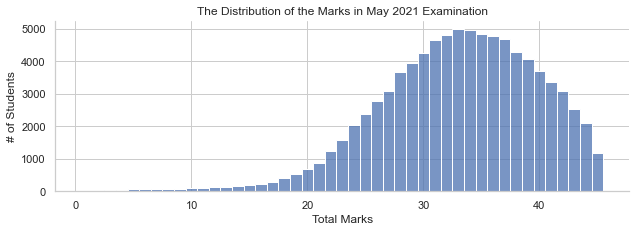
\includegraphics[width=\textwidth]{assets/maydist.png}
    \caption{The score distribution as recorded by IBO in the May examination, 2021}
    \label{fig:ibo_total}
\end{figure}

I know you are excited to see some data. Figure \ref{fig:ibo_total} shows the distribution of IB total scores as recorded by the IBO in the May 2021 examination.

Please note that the figure only represents one sample out of hundreds of past IB examinations, and therefore is heavily depended on recent events and in this case, global events. The result of a more detailed analysis is displayed in figure \ref{fig:maystat}.

\begin{marginfigure}
    \begin{lstlisting}[language=bash]
    count    87360.000000
    mean        33.005437
    std          6.808620
    min          2.000000
    25%         29.000000
    50%         33.000000
    75%         38.000000
    max         45.000000
    \end{lstlisting}
    \caption{The statistical description output of the IBO dataset}
    \label{fig:maystat}
\end{marginfigure}

The output shows that the dataset contains over 80,000 items, has a mean of 33 marks and a standard deviation of 6.8. Feel free to make your own interpretation of data for now.

In comparison, the data gathered from Year 12 Scots College students --- acting as the sampling data, graphed rather interestingly in figure \ref{fig:college_total}.
\begin{figure}
    \centering
    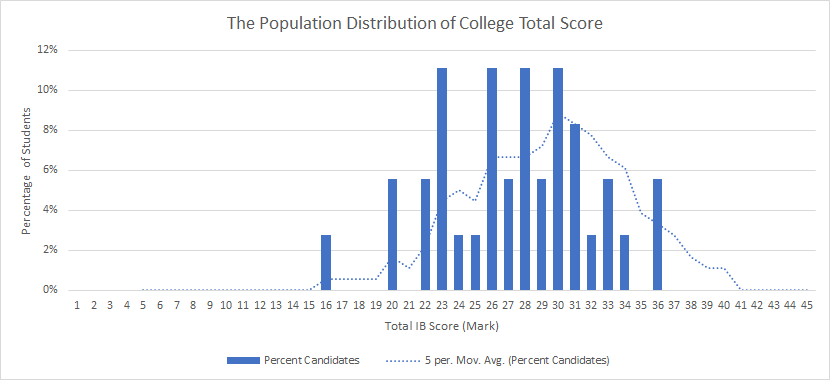
\includegraphics[width=\textwidth]{assets/college_total.png}
    \caption{The score distribution of Scots College students, Term 2 of 2021}
    \label{fig:college_total}
\end{figure}

The distribution is a lot more random than the IBO data --- as suspected from a sample size of 37 students. A moving average trendline has been included as an attempt to smooth-out the bars and reveal the trend. Let's look at this dataset more numerically in figure \ref{fig:dcol}.

\begin{marginfigure}
    \begin{lstlisting}[language=bash]
    count    37.000000
    mean     27.459459
    std       4.580118
    min      16.000000
    25%      24.000000
    50%      28.000000
    75%      30.000000
    max      36.000000
    \end{lstlisting}
    \caption{The statistical description output of the college dataset}
    \label{fig:dcol}
\end{marginfigure}

The above output shows that the collected dataset contains 37 values, with a mean of 27.5 marks and a standard deviation of 4.6 marks. Once again, make yourself at home with your own interpretations of these values.

\section{Data Collection}
The population data is retrieved from the IBO statistics page, where the most recent November and May examination results are taken for completeness. Although the college dataset is the population of students in Scots College, it is but merely a sample in terms of the IB as a whole. The sampling is not random, but rather focused on the college and Year 12 students\footnote{The keyword ``sample'' is used in two context: within the IB globally, and within the college. The dataset is not a sample of the college, but it is a sample of the IB population}. And as we are able to ``conduct'' a census on both the college and IB statistics, we fulfill any sample size requirement and guarantees a more accurate and precise analysis.

The steps of retrieving the college dataset is completed with the utilization of the school system. The overarching idea is to create a list of names of all Year 12 students, retrieve the grades from their report, and dumping everything into a database. The process is quite difficult in the planning, but looking back it is a lot easier and more accurate than a survey or a questionnaire --- because people lie in surveys. After the process, I am left with a .csv file with the respective information.

\section{Analysis}
% the dataset
\subsection{Dataset}

We will firstly focus on the college data, for there are some interesting relations embedded in these numbers. Generally saying --- by looking at figure \ref{fig:dcol}, the total scores have an low but not surprising standard deviation of $4.6$ marks. What is surprising for me is the low mean of $27.3$. For I have often heard (from students and from teachers), that the average score is around 31 at the end of the two years\footnote{This turns out to be true as the dataset of the official IBO have shown}. This is a reasonable score for many universities accept scores above and around 33 marks --- Auckland university, the university of Toronto, etc.

% general datasets
By grouping the collected data into subjects, we are able to make crude comparisons in the student's familiarity and abilities throughout a range of disciplines.

\begin{figure}
    \centering
    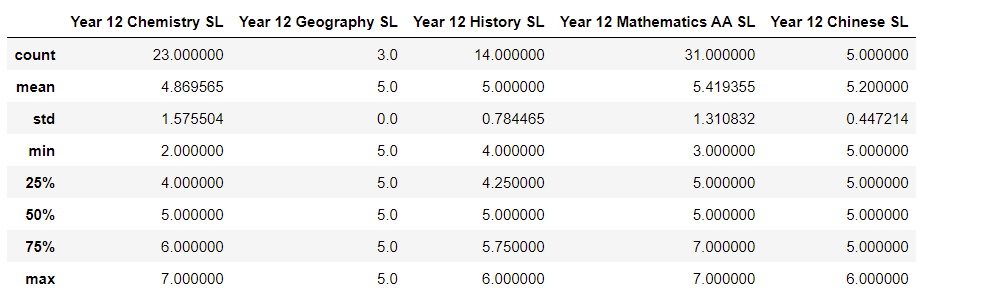
\includegraphics[width=\textwidth]{assets/col_sample.png}
    \caption{The statistical description output of 5 samples of the dataset}
    \label{fig:colsample}
\end{figure}

Figure \ref{fig:colsample} displays the statistics of a randomly chosen sample of 5 subjects\footnote{We only show five subjects because the paper is not wide enough to fit over 15 columns.}. Roughly we can make some deductions: that the Geography data has only 3 values, indicating a less representative and precise description; Mathematics AA stands out of the bunch by having the highest mean of $5.419$, and along with the largest sample size of 31, it is fair to say that many excel in maths in the college.

% whisker graph
In search of the general trend and to make comparisons between subjects, we will zoom out, and use multiple box plots to put subjects against one-another.

\begin{figure}
    \centering
    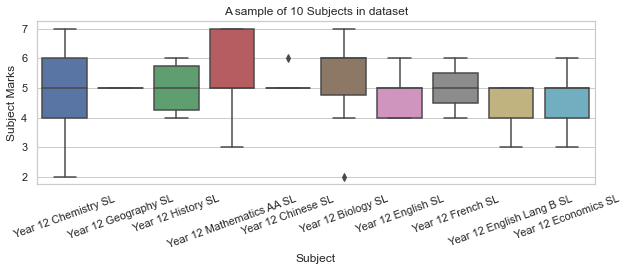
\includegraphics[width=\textwidth]{assets/subject_s0.png}
    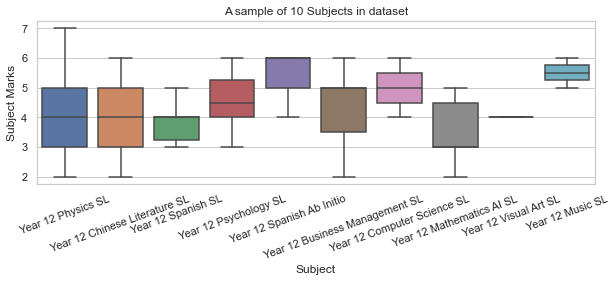
\includegraphics[width=\textwidth]{assets/subject_s1.png}
    \caption{Box plots of the subject marks in various subjects}
    \label{fig:subjects}
\end{figure}

By viewing the box plots\footnote{To read the box plot: the top ``whisker'' represents the maximum grade achieved in a subject, and the bottom whisker displays the lowest grade; the colored region represents the location of 50\% of data points, with the center line being the median value.} we are able to deduce some interesting facts. AA Mathematics seems to be the most well-y performed subject, for the colored region is placed the highest out of the bunch; Physics have the widest range of marks from 2 to 7 --- it has a high variance; Economics seems to have a higher and less variant mark then business, even though students have often told me they perceive the latter being easier than the former; only 4 subjects gifted 7s to students, and only 5 subjects gifted 2s to students; and lastly, the median marks for all subjects seems to hover around 4 and 5.

This statistic could be useful to course organizers and teachers, for these ``facts'' can tell a story. For example, AA maths performed better than AI maths. Teachers can use this finding to focus resources on AI maths if the school wishes to appeal to all students; Spanish ab inito have higher average marks than the Spanish course. This might trigger a investigation into the difficulty of these similar courses as we expect similar if not better performance for the experienced Spanish learners. The point I am bringing is that statistics like these, even if not representative of personal ability, can give off subtle hints that can be caught and improved upon.

% maths & literiture
\subsection{Correlation}

With the big picture in mind, by digging deeper we can uncover more interesting statistics and graphs.

\begin{marginfigure}
    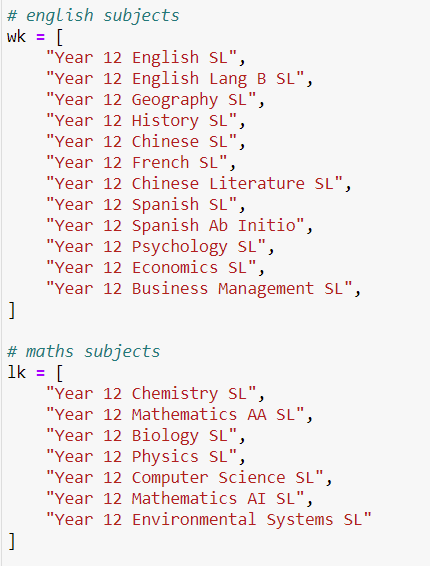
\includegraphics[scale=0.5]{assets/wklk.png}
    \caption{My decision on the list of English and Maths subjects}
\end{marginfigure}

\begin{figure}
    \centering
    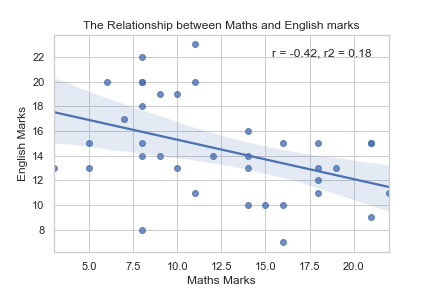
\includegraphics[width=\textwidth]{assets/maths_english.png}
    \caption{Scatter plot with regression line between Maths and English subject scores}
    \label{fig:mathenglish}
\end{figure}

I am uncertain in other languages, but subjects are split into two primary ``disciplines'' in China --- English and Maths, roughly. It may be interesting to visualize the relationship between marks the students have gained in these areas. Here in figure \ref{fig:mathenglish} I have graphed the relationship between the two areas in the form of a scatter plot.

There seems to be a negative correlation between the two fields: students with higher total Maths marks received generally lower total English marks, vice versa. This is likely due to human nature preferring one area over another and thus performing better, and therefore justifying the categorization in the first place.

However, as indicated by the dim regions around the trend line, there exists a lot of uncertainty. This is exampled by the low coefficient of determination ($r^2 = 0.18$)  of the regression line, which means that not a lot of variation in the English scores is explained with the knowledge of Maths marks. Thus, we should be critical in the confidence we have in presenting this result to the college as we are not confident in the accuracy of the relation.

Additionally\footnote{There is someone I need to thank here, for he had pointed this out}, this is one area  where statistics can become misleading if taken at face-value.

\begin{figure}
    \centering
    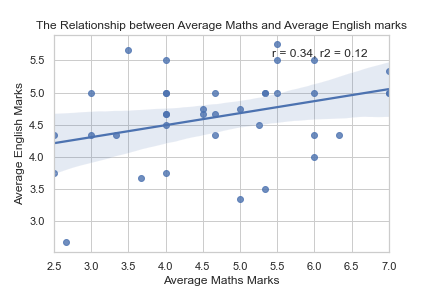
\includegraphics[width=\textwidth]{assets/avg_maths_english.png}
    \caption{Scatter plot with regression line between Average Maths and Average  English subject scores}
    \label{fig:mathenglishavg}
\end{figure}

If we simply average the scores with the number of courses taken, as shown in figure \ref{fig:mathenglishavg}, the correlation is flipped in the opposite direction. This is not surprising, for the negative correlation in figure \ref{fig:mathenglish} can also be explained in that more English courses $=$ less Maths courses, and vice versa. Therefore the total marks will be inversely related even if there are no actual correlations. Within the average graph, there is a very loose positive correlation with a $r^2$ of $0.12$. It can be tempting to say that higher English grades means higher Maths grades.

\subsection{Comparison}

% comparing with IBO
Finally, we will conclude this analysis with the comparison between the global and college datasets. We shall consider three datasets: 2020 November examination, 2021 May examination, and our collected statistics. By including the most recent and a broad range of data, we allow for fairer and more meaningful comparisons.

\begin{figure}
    \centering
    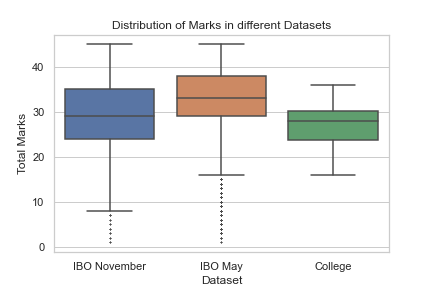
\includegraphics[width=\textwidth]{assets/total.png}
    \caption{The distribution of total marks among the May, November, and sampled datasets}
    \label{fig:dist}
\end{figure}

Figure \ref{fig:dist} shows the box plot of the three datasets. At a glance, we can see that the May exam had the highest median mark, followed by the November exam, then the College results. A reasonable explanation is that the northern hemisphere is more try-hard then the southern.

Additionally, notice the smaller variance in the college statistics comparing to the exams. This is explained statistically, as our college data is a sample of the population exam data. Naturally by taking samples, the samples are more likely to be taken from around the mean, hence closer data points and a lower variance.

We conclude by stating that the College statistics are more similar to the November's Exams then to the May's, which should pose little concern to the school for the students are performing as expected --- more or less near average.

\section{Testing}
% talk about testing
A hypothesis test is used in statistics to determine whether a sample is taken from a target population by testing its sample mean. We can conduct such tests on our data against the 2021 May examination statistics as well as the 2020 November examination. Ideally, we would see that our data is more likely to have originated from the November exam, for that is the exam Scots College students take.

Via computation, we can find the mean and variance of the three datasets:
\begin{align*}
    \text{May:}\,\, &\mu = 33.0, \,\sigma = 6.82, \,n = 87372\\
    \text{November:}\,\, &\mu = 29.6, \,\sigma = 7.60, \,n = 15222\\
    \text{Sample:}\,\, &\mu = 27.5, \,\sigma = 4.51, \,n = 37
\end{align*}
We can also visualize the datasets with the assumption that they are all normally distributed\footnote{Yes, the distribution of data as shown in the first figure is left skewed; Yes, the distribution extends above 45; Yes, this means that the result might not be accurate. But since the mean is not too close to the range limits, and the upper limit is at least two standard deviation away, means that for the sake of the analysis, this assumption of a normal distribution is a reasonable one}:

\begin{figure}
    \centering
    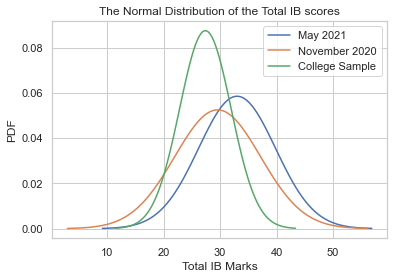
\includegraphics[width=\textwidth]{assets/dist.png}
    \caption[][6cm]{The distributions of the datasets}
    \label{fig:ddist}
\end{figure}
It is obvious by viewing figure \ref{fig:ddist} that the college sample is more closely related to the November dataset than the May, but by how much and how significant is that? We will use a hypothesis test for each pair to determine the significance.

% discuss the two tests
Let us first analyze the relationship between the May and the college datasets. We start by defining our null and alternative hypothesis, represented by $H_0$ and $H_1$. The null hypothesis is often the one of least concern, and the alternative hypothesis is the result one is looking for. In this case:
\begin{align*}
    H_0 &: \mu = \mu_{\text{may}}\\
    H_1 &: \mu < \mu_{\text{may}},
\end{align*}
for the significant result is that the college performed worse. The test will lead us either to accept the null hypothesis or to reject it, and accept the alternative hypothesis. We also need an alpha level, or the significance level that controls the probabilities of a Type I error --- the chance of us having a false positive and rejecting the null hypothesis when it is actually true. I had chosen a standard alpha level of $0.01$ or $1\%$, as I want the result to be of more certainty.

The basis of the test is to see if our sample mean is far enough away from the sampling distribution of the sample mean that there is only an $\alpha$ probability for a Type I error. The cutoff point is deemed the critical value, for which we will show the process of calculating it below.

Let $X$ be a random variable representing the distribution of student's score in the May examination. We assume that X is normally distributed, thus:
\begin{align*}
    X &\sim N(33.0, 6.82^2)\\
    \overline{X} &\sim N(33.0, \frac{6.82^2}{37}).
\end{align*}

Let $c$ be the critical value for this one-tail test --- that we are only looking for if the sample population mean is less than the population mean. Therefore:
\begin{align*}
    P(\overline{x} < c) &= \alpha = 0.01\\
    c &= 30.4.
\end{align*}

We name our $\overline{x}$ the test statistics. For we did not normalize our population data, our test statistics is the sample mean of $27.5$. With these number, we can reject our null hypothesis as $\overline{x} < c$ for our test statistics resides in the rejection region, meaning that we will instead accept the alternative hypothesis --- that our sample is not sampled from the May dataset as they differ largely in sample mean.

The test can also be applied to the November dataset, the steps are as follows.

We set up our null and alternative hypothesis:
\begin{align*}
    H_0 &: \mu = \mu_{\text{november}}\\
    H_1 &: \mu < \mu_{\text{november}},
\end{align*}
then using an alpha level of $0.01$, the critical value $c$ is:
\begin{align*}
   P(\overline{x} < c) &= \alpha = 0.01\\
   c &= 26.7.
\end{align*}
For our sample statistics (sample mean) is larger than the critical value, it is in the accepting region. So we accept our null hypothesis, and conclude that the sample originated from the November dataset.

% what we can make from it
With the two tests, we can conclude with high confidence that our college dataset originated from the November dataset, but not from the May dataset. This is understandable as the students are from the southern hemisphere and take their exams in November as well. In fact, the dataset is certain to contain previous Year 13 students scores from this school. This lack of unexpected results means that the school may not need to consider any deliberate actions, and that their current method of teaching is satisfactory in making the average.

\section{Final Words}
% what we have experimented with and how it hows the school to make decisions
In this report, we used the collected Scots College Year 12 Term 2 dataset and compared it against examination scores, as well as itself. We've looked at the distribution of the scores, and compared the marks throughout the subjects; We analyzed the relationship between Maths and English marks, and went further in deciding that the test was erroneous; Finally, we compared the sample datasets against the examination results, and had conducted two hypothesis tests to determine the relationship between our samples and the examinations. Throughout the sections, we have mentioned the insights gained from the comparisons, and to which I sincerely hope, that the college can make the full use of.


\end{document}
